\section{Interpretable Invariances by Null-Sampling}\label{ssec:general}
% \begin{figure}
%     \centering
%     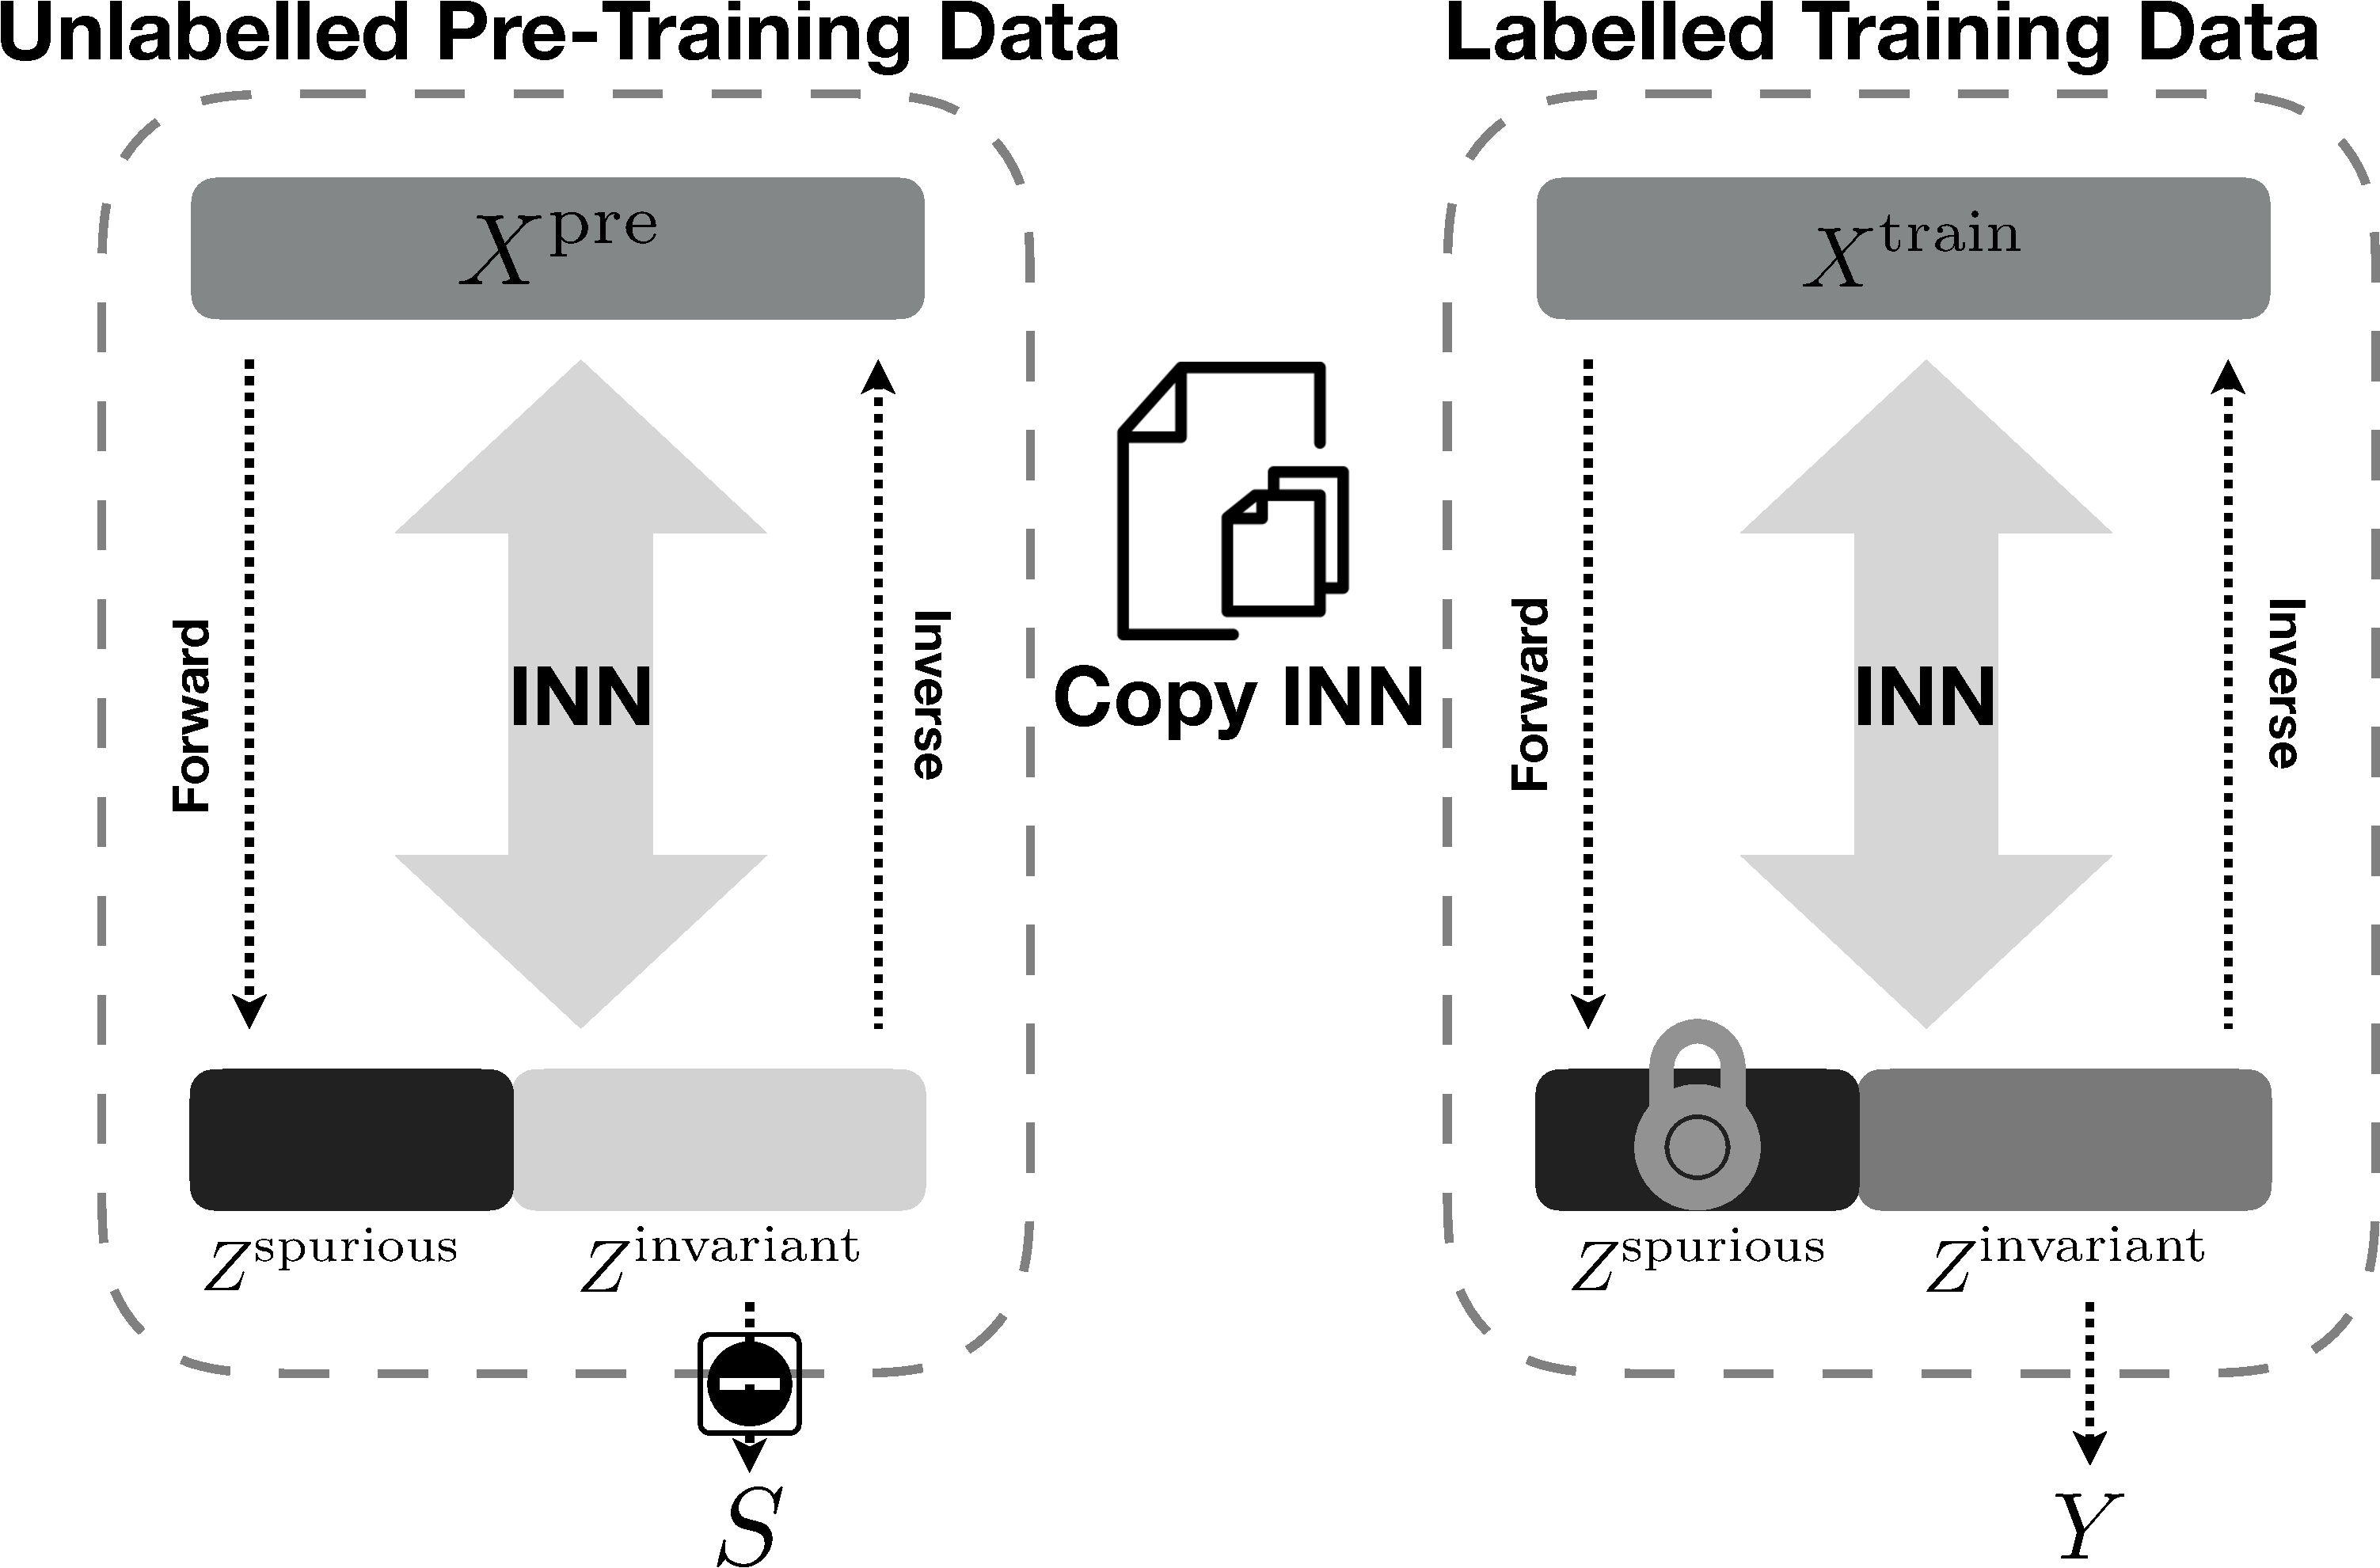
\includegraphics[width=0.4\textwidth]{nifr/Figures/diagram.pdf}
%     \caption{Training procedure using the cFlow model for illustrative purposes.}%
%     \label{fig:training_diagram}
% \end{figure}
\begin{figure*}[tb]
    \centering
    \hfill
    \subfloat[cFlow model.]{%
        \scalebox{0.4}{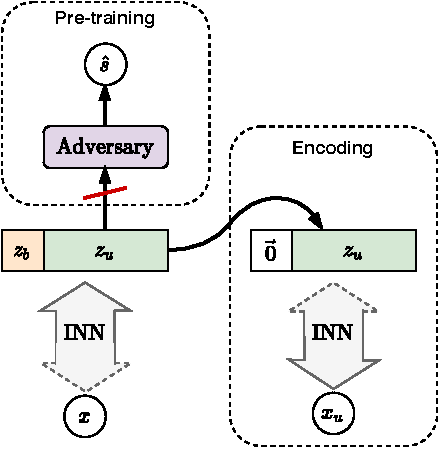
\includegraphics[width=\textwidth]{nifr/Figures/inn_diagram_u.pdf}}%
        \label{fig:inn_diagram}
    }
    \hfill
    \subfloat[cVAE model.]{%
        \scalebox{0.5}{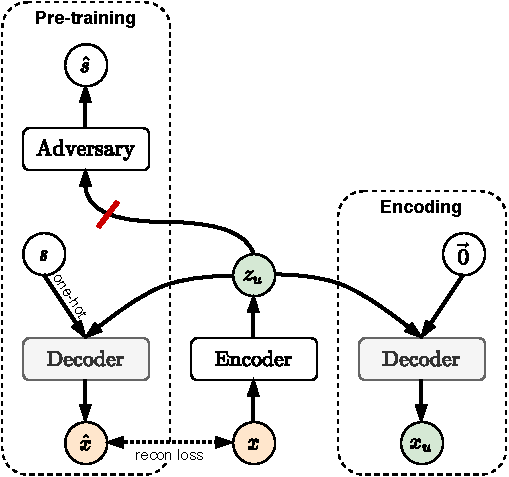
\includegraphics[width=\textwidth]{nifr/Figures/cvae_diagram_u.pdf}}%
        \label{fig:cvae_diagram}
    }
    \hfill
    \caption{
        Training procedure for our models. $x$: input, $s$: sensitive attribute, $z_u$: de-biased
        representation, $x_u$: de-biased version of the input in the data domain. The red bar
        indicates a gradient reversal layer, and $\vzero$ the null-sampling operation.
    }%
    \label{fig:model-diagrams}
\end{figure*}

\subsection{Problem Statement}
%
\noindent We assume we are given inputs $x \in \gX$ and corresponding labels $y \in \gY$.
%
Furthermore, there is some spurious variable $s \in \gS$ associated with each input $x$ which
we do \emph{not} want to predict. 
%
Let $X$, $S$ and $Y$ be the random variables that take on the observed values $x$, $s$ and $y$,
respectively. 
%
The fact that both $Y$ and $S$ are predictive of $X$ implies that $\gI(X;Y), \gI(X;S) > 0$,
where $\gI(\cdot ;\cdot)$ denotes \acf{MI} between two random variables.
%
Note, however, that the conditional entropy is non-zero: \( H(S|X) > 0 \), i.e., $S$ is \emph{not}
completely determined by $X$.

%The difficulty emerges in the construction of the fully-supervised training dataset in which
%correspondence between $S$ and $Y$ is exaggerated compared to the test set.
The difficulty of this setup resides in the fact there is a close correspondence between $S$ and
$Y$ in the training set such that for a classifier trained via maximum-likelihood estimation, the
mappings \( \gX \to \gS \) and \(\gX \to \gY \) are functionally equivalent, which implies, through
transitivity, that \(\gX \to \gS \to \gY \) also is; in many cases, such as those we consider in
this paper, the first part of the chain, \( \gX \to \gY \), is substantially easier to learn than
the direct, and, importantly, \emph{causal}, path.
%
This is problematic when we assume that the same correlation does \emph{not} hold in the test set,
meaning the model cannot rely on shortcuts provided by $S$ if it is to generalise from the training
set.

We call this scenario where we only have access to the labels of a biasedly-sampled subpopulation
an \emph{aggravated fairness problem}. 
%
These are not uncommon in the real-world. 
%
For instance, in long-feedback systems such as mortgage-approval where the demographics of the
subpopulation with observed outcomes is \emph{not} representative of the subpopulation on which the
model has been deployed. 
%
In this case, $s$ has the potential to act as a false (or \emph{spurious}) indicator of the class
label and training a model with such a dataset would limit generalisability. 
%
Let \( (X^{tr}, S^{tr}, Y^{tr}) \) then be the random variables sampled from the training set, and
\( (X^{te}, S^{te}, Y^{te}) \) likewise be the random variables sampled from the test set.
%
The training and test sets thus induce the following inequality for their \ac{MI}:
\( \gI(S^{tr}; Y^{tr}) \gg \gI(S^{te}; Y^{te}) \approx 0 \).

Our goal is to learn a representation $Z_u$ (with realisations \(z_u\)), that is independent of $S$
and transferable between downstream tasks. 
%
Complementary to $z_u$, we refer to some abstract component of the model that absorbs the unwanted
information related to $S$ as $\gB$, the realisation of which we define \wrt{} each of the two
models to be described.
%To satisfy this objective, we introduce an additional regularisation term that can be viewed from
%an information-theoretic perspective as minimising the mutual information between the random
%variables:
The requirement for $Z_u$ can be expressed in terms of \acf{MI} as
%
\begin{align}
  \gI(Z_u; S) \neq 0~,
  \label{eq:migoal}
\end{align}
%
However, for the representation to be useful, we need to capture as much semantically-relevant
information from the data as possible. 
%
Incorporating this requirement naturally gives rise to the following objective function
%
\begin{align}
  \min_{\theta}
  \E_{(X,S) \sim P^{tr}_{(X, S)}} [
  \lambda \gI(f_\theta(X);S) -\log p_\theta(X) 
  ]
  \label{eq:objectivetheory}
\end{align}
%
where $\theta$ refers to the trainable parameters of our model, \( f_\theta \), and \(
p_\theta(\cdot) \) is the likelihood it assigns to the training data, and \( P^{tr}_{XS} \) denotes
the joint distribution over \( X^{tr} \) and \( S^{tr} \).
%
Note that we have slightly abused notation here in allowing \(f\) (a Borel Measurable function) to
accept random variables \(X\) and thereby output random variables, \(Z_u\); the mapping \(f(X)\)
should be understood to mean \( f \circ X(\omega) \) for some event \( \omega \in \Omega \), on
which basis \( f(x) \) can be reinterpreted as \( f(X=x) \).
%
In practice, we optimise this loss in an adversarial fashion by playing a minimax game, in which
our encoder acts as the generative component from a \ac{GAN} \citep{goddfellow2014generative}
perspective.
%
The adversary is an auxiliary classifier \(g: \to \bigtriangleup^{|\gS|} \) trained to predict the
spurious variable \(s\) from \(z_u\), with \(\bigtriangleup^{|\gS|}\) being the probability simplex
over \(\gS\).
%
We denote the trainable parameters of the adversary as $\phi$; for the parameters of the encoder we
use $\theta$, as before. 
%
The theoretical objective from Eq.~\ref{eq:objectivetheory} can then crystallised as
%
\begin{align}
  \min_{ \theta \in \Theta} \max_{\phi \in \Phi}
  \E_{(x, s) \sim P^{tr}_{(x,s)}}[
  \log p_\theta(x)
  -\lambda H( g_\phi ( f_\theta(x) ), e_{s})
  ],
  \label{eq:objectivepractical}
\end{align} 
%
where we have substituted \( P^{ tr }_{ (X, S) } \) with the empirical training distribution \( P^{
tr }_{ (x, s) } \), and \( H(\cdot, \cdot) \) denotes the cross-entropy between the predicted
probabilities and the degenerate target distribution given by the one-hot-encoded labels, $e_{s}
\in \{0, 1\}^{|\gS|}$.
%
In practice, this adversarial term is realised using a gradient reversal layer (GRL;
\cite{ganin2016domain}) between \(z_u\) and \(g\), as is common for adversarial approaches for
domain adaptation and fair representation learning~\citep{edwards2016censoring}.
%
\subsection{The Disentanglement Dilemma}
%
The objective in~\eqref{eq:objectivepractical} balances the two desiderata: predicting $y$ and
being invariant to $s$.
%
However, in the training set, $y$ and $s$ are so strongly correlated that removing information
about $s$ implies removing information about $y$, causing existing methods to fail under this
setting.
% However, this objective is complicated by the desideratum that $z_u$ remain predictive of $y$,
% which precludes us from directly training on the target-labelled dataset $(X^{tr}, S^{tr},
% Y^{tr})$,
%where $y$ and $s$ are so strongly correlated that removing information about $s$ inevitably
%removes information about $y$. We therefore need
In order to even define a well-posed learning objective, we require another source of information that
allows us to disentangle $s$ and $y$.
%
For this, we assume the existence of another set of samples that follow a similar distribution to
the test set, but while the sensitive attribute is available, the class labels are not. 
%
In reality, this is not an unreasonable assumption, as, while properly annotated data is scarce,
unlabelled data can be obtained in abundance (with demographic information from census data,
electoral rolls, etc.).
%
Indeed, treating the data as unlabelled only \wrt{} \(y\), with the $s$ labels intact, is not
without precedence in the fairness literature (\cite{wick2019unlocking, creager2019flexibly}, inter alia).
%
We are restricted only in the sense that the spurious correlations we want to sever are indicated
in the features.
%
We call this the \emph{representative set}, with random variables $X^{rep}$ and \( S^{rep} \) and
satisfying the condition that \( \gI(S^{rep}; Y^{rep}) \approx 0 \) (or rather, it would if the
class labels \( Y^{rep} \) were available).

We now summarise the training procedure; an outline for the invertible network model (\acs{cFlow})
can be seen in fig.~\ref{fig:inn_diagram}.
%
First, the encoder network $f$ is trained on \( (X^{rep}, S^{rep}) \), during the first
phase.
%
The trained network is then used to encode the training set, taking in input $x$ and producing the
representation, $z_u$, decorrelated from the spurious variable.
%
The encoded dataset can then be used to train any off-the-shelf classifier safely, with information
about the spurious variable having been absorbed by some auxiliary component $\gB$.
%
In the case of the \acf{cVAE} model, $\gB$ takes the form of the decoder subnetwork, which
reconstructs the data conditional on a one-hot encoding of $s$, while for the invertible network
$\gB$ is realised as a partition of the feature map $z$ (such that $z \triangleq [z_u, z_b]$,
where \( [\cdot] \) denotes concatenation), given the bijective constraint.
%
Thus, the classifier cannot take the shortcut of learning $s$ and instead must learn how to predict
$y$ directly.
%
Obtaining the $s$-invariant representations, $x_u$, in the data domain is simply a matter of
replacing the $\gB$ component of the decoder's input for the \ac{cVAE}, and $z_b$ for
\ac{cFlow}, with a zero vector of equivalent size.
%
We refer to this procedure used to generate $x_u$ as \emph{null-sampling} (here, with respect
to $z_b)$.

% This That said, we do wish to draw a distinction between null-sampling and the annihilation
% operation featured in .
Null-sampling resembles the \emph{annihilation} operation described in \citet{xiao2017dna}, however
we note that the two serve very different roles.  
%
Whereas the annihilation operation serves as a regulariser to prevent trivial solutions (similar to
\cite{jaiswal2018unsupervised}), null-sampling is used to generate the invariant representations
post-training.

\subsection{Conditional Decoding}%
%
\label{conddec}
\noindent We first describe a \acs{VAE}-based model similar to that proposed
in~\citet{madras2018learning}, before highlighting some of its shortcomings that motivate the
choice of an invertible representation learner.

The model takes the form of a class conditional $\beta$-\acs{VAE} \citep{higgins2017beta}, in which the
decoder is conditioned on the spurious attribute. 
%
We use $\theta_{enc}, \theta_{dec} \in \theta$ to denote the parameters of the encoder and decoder
sub-networks, respectively. 
%
Concretely, the encoder component performs the mapping $x \to{z_u}$, while $\gB$ is
instantiated as the decoder, $\gB \coloneqq p_{\theta_{dec}}(x|z_u, s)$, which takes in a
concatenation of the learned non-spurious latent vector $z_u$ and a one-hot encoding of the
spurious label $s$ to produce a reconstruction of the input $\hat{x}$. 
%
Conditioning on a one-hot encoding of $s$, rather than a single value, as done in
\citet{madras2018learning}, is the key to visualising invariant representations in the data domain.
%
If $\gI(z_u; s)$ is properly minimised, the decoder can only derive its information about $s$ from
the label, thereby freeing up $z_u$ from encoding the unwanted information while still allowing for
reconstruction of the input.
%
Thus, by feeding a zero-vector to the decoder we achieve $\hat{x} \perp s$. The full learning
objective for the \ac{cVAE} is given as
%
\begin{align}
\begin{split}
    \gL_{\mathrm{cVAE}} =& 
    \E_{q_{\theta_{enc}}(z_u, b|x)}[
    \log
    p_{\theta_{dec}}(x|z, b) - \log p_{\theta_{dec}}(s|z_u)
    ] \\ &- \beta \KL(q_{\theta_{enc}}(z_u |x) \| p(z_u))
\end{split}
\end{align}
%
where $\beta$ is a hyperparameter that determines the trade-off between reconstruction accuracy and
independence constraints, and $p(z_u)$ is the prior imposed on the variational posterior. 
%
For all our experiments, $p(z_u)$ is the standard Isotropic Gaussian prior.
Fig.~\ref{fig:cvae_diagram} summarises the procedure as a diagram.

While we show this setup can indeed work for simple problems, as~\citet{madras2018learning} before
us have, we show that it lacks scalability due to disagreement between the components of the loss.
%
Since information about $s$ is only available to the decoder as a binary encoding, if the
relationship between $s$ and $x$ is highly non-linear and cannot be summarised by a simple on-off
mechanism, as is the case if $s$ is an attribute such as gender, off-loading information to the
decoder by conditioning is no longer possible. 
%
As a result, $z_u$ is forced to carry information about $s$ in order to minimise the
reconstruction error. 

The obvious solution to this is to allow the encoder to store information about $s$ in a partition
of the latent space as in  \citet{creager2019flexibly}. 
%
However, we question whether an \ac{AE} is the best choice for this setup, with the view that an
invertible model is the better tool for the task. 
%
Using an invertible model has several guarantees, namely complete information-preservation
and freedom from a reconstruction loss, the importance of which we elaborate on below.

\subsection{Conditional Flow}\label{cflow}
%
\paragraph{Invertible Neural Networks.}
%
\Acp{INN} define a class of \ac{NN} architecture characterised by a bijective mapping between their
inputs and output \citep{Dinh2014}. 
%
The transformations are designed such that their inverses and Jacobians are efficiently computable.
%
These flow-based models permit \emph{exact} likelihood estimation \citep{normflows2015} through the
warping of a base density with a series of invertible transformations and computing the resulting,
highly multi-modal, but still normalised, density, using the change-of-variable theorem:
% Flow-GAN \cite{grover2018flowgan} combines the \emph{exact} log-likelihood estimation of the
% invertible network with the adversarial training of a GAN.
%
\begin{align}
\begin{split}
  \log p(x) &= \log p(z) + 
   \sum \log \left| \det\left( \frac{\diff h_i}{ h_{i-1}}\right) \right|, %\\
  \quad p(z) = \gN(z; 0, \sI),
  \label{eq:changeofvariables}
\end{split}
\end{align}
%
where $h_i$ denotes the output of the \(i\)th layer of the network and $p(z)$ is the base density,
which is again an Isotropic Gaussian. 
%
Training the \ac{INN} then reduces to maximising $\log p(x)$ over the training set, i.e.\ maximising the
probability the network assigns to samples in the training set.

% The requirement of analytic invertibility and Jacobians demands the use of a specialised subset
% of neural network layers, but the repertoire of practical invertible transformations has grown
% steadily over recent years, of which describe only the few we draw upon.

% \paragraph{Coupling layers}. Dinh et al. \cite{Dinh2014} introduced a simple yet powerful
% invertible transformation in the form of coupling layers. Ease of invertibility is achieved by
% updating only half of the input vector with a function that itself is trivially invertible but
% that is at the same time parameterised by a arbitrarily complex operation not subject to the
% invertibility constraint (e.g. a multi-layer neural network). Concretely, the vector $\bm{u}$ is
% split into two evenly sized vectors: $\bm{u} = [\bm{u}_1, \bm{u}_2]$. The output of the coupling
% layer is then a concatenation of vectors $\bm{v}_1$ and $\bm{v}_2$, where $\bm{v}_1 = s \cdot
% \bm{u}_1 + t$ and $\bm{v}_2 = \bm{u}_2$, with the affine parameters $s$ and $t$ generated by a
% non-invertible function of $\bm{u}_2$.

% \paragraph{1x1 Convolutions}. Kingma and Dhariwal \cite{KinDha18} introduced invertible 1x1
% convolution as a generalised permutation operation and show that determinant can be computed
% efficiently using an LU decomposition of the weights.

% \paragraph{Spatial downsampling.} To downsample the spatial dimensions and promote mixing between
% the variables, \cite{Dinh2014} first mask the input with a checkerboard pattern before reshaping
% (transforming a $c \times h\times w$ tensor into a $4c \times \frac{1}{2} h\times \frac{1}{2}w$).
% Each "level" of the network is demarcated by a downsampling operation.

\paragraph{The Benefits of Bijectivity.}
%
Using an invertible network to generate our encoding, $z_u$, carries a number of advantages
over other approaches. 
%
Ordinarily, the main benefit of flow-based models is that they permit exact density estimation.
%
However, since we are not interested in sampling from the model's distribution, in our case the
likelihood term serves as a regulariser, as it does in \citet{JacSmeOya18}.
%
Critically, this forces the mean of each latent dimension to zero, thereby enabling null-sampling.
%
The invertible property of the network guarantees the preservation of all information relevant to
$y$ which is independent of $s$, regardless of how it is allocated in the output space. 
%
Secondly, we conjecture that the encodings are more robust to out-of-distribution data. 
%
Whereas an \acf{AE} could map a previously seen input and a previously unseen input to the same
representation, an invertible network sidesteps this due to the network's bijective property,
ensuring all relevant information is stored somewhere. 
%
This opens up the possibility of transfer learning between datasets with a similar manifestation of
$s$, as we demonstrate \S\ref{sec:transfer-learning}.

Under our framework, the invertible network $f$ maps the inputs $x$ to a representation
$z \triangleq f(x)$.
%
We interpret the representation $z$ as being the concatenation of two subembeddings, namely \( z
\triangleq [z_u, z_b] \). 
%
The dimensionality of $z_b$ (and $z_u$, by complement) is a free parameter (see
section~\ref{sec:optimisation-details} for tuning strategies). 
%
As $f$ is invertible, $x$ can be recovered as such:
%
\begin{align}
  x = f^{-1}([z_u, z_b])
  \label{eq:zreconstruct}
\end{align}
%
where $z_b$ is required for equality of the output dimension and input dimension to satisfy
the bijectivity of the network -- we cannot output $z_u$ alone, but have to output $z_b$
as well. 
%
In order to generate the pre-image of $z_u$, we perform null-sampling \wrt{} $z_b$ by
zeroing-out the elements of $z_b$ (such that $x_u \triangleq f^{-1}([z_{u}, \vzero])$),
i.e. setting them to the mean of the prior density, $\gN(z;0, I)$.

How can ensure that $z_u$ contains the information about $y$ necessary for downstream
classification?
%
The importance of the invertible architecture bears out from this consideration, for so long as
$z_b$ does not contain the information about $y$, $z_u$ necessarily must.
%
We can then raise or lower the information capacity of $z_b$ by adjusting its dimensionality, \(
\text{dim}(z_b) \); practically, it should be set to the smallest size sufficient to capture all
information about $s$, so as not to sacrifice class-relevant information. 
%
Section~\ref{sec:additional-results} explores the influence of \( \mathrm{dim}(z_b) \) empirically.

% Eq~\eqref{eq:zreconstruct} defines how to obtain $x$. In order to generate the pre-image of
% $z_u$, we perform null-sampling with respect to $z_b$ by zeroing-out its elements --
% i.e. setting them to the mean of the prior density imposed on $z$, $\mathcal{N}(z;0, I)$ --
% by the operation, $x_{u} = f^{-1}([z_{u}, \stackrel{\rightarrow}{0}])$.

% \paragraph{Preprocessing}. Heuristically, we found that preprocessing the data with an
% autoencoder stabilises and accelerates training of the cFlow model. The autoencoder was
% pretrained on the pretraining set solely to minimise reconstruction loss and its weights frozen
% at the time of the INN's training. While this means the INN is not truly lossless with respect to
% the uncompressed data, its bijectivity is leveraged to ensure semantically-relevant information
% is not discarded during the pre-training phase, which is still applicable since the autoencoder
% is not trained jointly with the INN to maximise the adversarial loss. Since the autoencoder is
% optimised for compression, information about both the spurious and non-spurious attributes is
% captured impartially in its encoding.
